% Reconstructed from the supplied mathematics test photographs.
% Requires tikz and the arrows.meta library.  No font definitions.
% Orthographic voxel projection: x right, y rear, z up.
% All internal faces are removed. Exterior faces are painter-sorted by
% exact overlap/depth comparisons, so occluded cube edges are not exposed.
\newcommand{\LocationMap}{%
\begin{tikzpicture}[x=8.3mm,y=8.3mm,line cap=round,line join=round,font=\small]
  \draw[step=1,black!65,line width=.32pt] (0,0) grid (5,4);
  \draw[-{Latex[length=1.45mm,width=1.1mm]},line width=.55pt] (0,0) -- (5.35,0);
  \draw[-{Latex[length=1.45mm,width=1.1mm]},line width=.55pt] (0,0) -- (0,4.3);
  \foreach \xx in {0,1,2,3,4,5}
    \node[below=2pt,font=\scriptsize] at (\xx,0) {\xx};
  \foreach \yy in {1,2,3,4}
    \node[left=2pt,font=\scriptsize] at (0,\yy) {\yy};
  \draw[line width=.8pt] (0,0) -- (3,3)
    node[pos=.5,sloped,above=2.5pt,fill=white,inner sep=.8pt,font=\scriptsize] {200米};
  \draw[line width=.4pt] (0,.75) arc[start angle=90,end angle=45,radius=.75];
  \node[fill=white,inner sep=.4pt,font=\scriptsize] at (.32,.88) {$45^\circ$};
  \fill (0,0) circle (1.3pt);
  \node[anchor=east,inner sep=0pt] at (-.25,-.29) {学校};
  \fill (2,3) circle (1.3pt);
  \node[above left=2pt,inner sep=0pt] at (2,3) {书店};
  \fill (3,3) circle (1.3pt);
  \node[above right=2pt,inner sep=0pt] at (3,3) {商店};
  \fill (3,2) circle (1.3pt);
  \node[below right=2pt,inner sep=0pt] at (3,2) {公园};
  \draw[-{Latex[length=1.6mm,width=1.1mm]},line width=.65pt]
    (5.65,3.15) -- (5.65,4.2) node[above=2pt,inner sep=0pt] {北};
\end{tikzpicture}%
}

\newcommand{\SolidChoices}{%
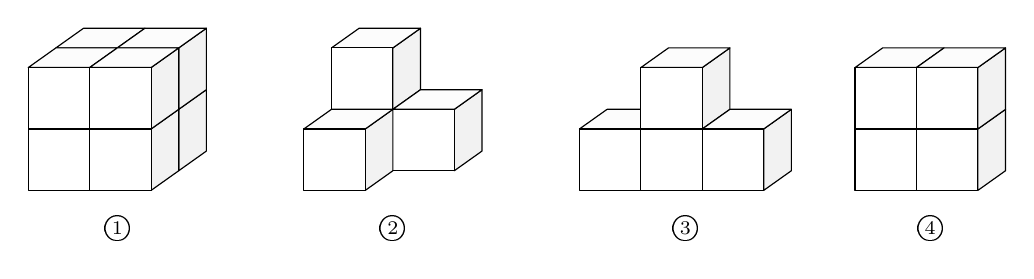
\begin{tikzpicture}[x=7.8mm,y=7.8mm,line cap=round,line join=round,line width=.42pt]

  \begin{scope}[xshift=0mm]
  \path[draw=black,fill=black!1] (0.45,2.32) -- (1.45,2.32) -- (1.9,2.64) -- (0.9,2.64) -- cycle;
  \path[draw=black,fill=black!5] (2.45,0.32) -- (2.9,0.64) -- (2.9,1.64) -- (2.45,1.32) -- cycle;
  \path[draw=black,fill=black!5] (2.45,1.32) -- (2.9,1.64) -- (2.9,2.64) -- (2.45,2.32) -- cycle;
  \path[draw=black,fill=black!1] (1.45,2.32) -- (2.45,2.32) -- (2.9,2.64) -- (1.9,2.64) -- cycle;
  \path[draw=black,fill=black!1] (0,2) -- (1,2) -- (1.45,2.32) -- (0.45,2.32) -- cycle;
  \path[draw=black,fill=black!5] (2,0) -- (2.45,0.32) -- (2.45,1.32) -- (2,1) -- cycle;
  \path[draw=black,fill=black!5] (2,1) -- (2.45,1.32) -- (2.45,2.32) -- (2,2) -- cycle;
  \path[draw=black,fill=black!1] (1,2) -- (2,2) -- (2.45,2.32) -- (1.45,2.32) -- cycle;
  \path[draw=black,fill=white] (0,0) -- (1,0) -- (1,1) -- (0,1) -- cycle;
  \path[draw=black,fill=white] (0,1) -- (1,1) -- (1,2) -- (0,2) -- cycle;
  \path[draw=black,fill=white] (1,0) -- (2,0) -- (2,1) -- (1,1) -- cycle;
  \path[draw=black,fill=white] (1,1) -- (2,1) -- (2,2) -- (1,2) -- cycle;
  \node[below=0pt,font=\small] at (1.45,-.35) {\textcircled{\scriptsize 1}};
  \end{scope}
  \begin{scope}[xshift=35mm]
  \path[draw=black,fill=black!5] (1.45,1.32) -- (1.9,1.64) -- (1.9,2.64) -- (1.45,2.32) -- cycle;
  \path[draw=black,fill=black!1] (0.45,2.32) -- (1.45,2.32) -- (1.9,2.64) -- (0.9,2.64) -- cycle;
  \path[draw=black,fill=black!5] (2.45,0.32) -- (2.9,0.64) -- (2.9,1.64) -- (2.45,1.32) -- cycle;
  \path[draw=black,fill=black!1] (1.45,1.32) -- (2.45,1.32) -- (2.9,1.64) -- (1.9,1.64) -- cycle;
  \path[draw=black,fill=white] (0.45,1.32) -- (1.45,1.32) -- (1.45,2.32) -- (0.45,2.32) -- cycle;
  \path[draw=black,fill=white] (1.45,0.32) -- (2.45,0.32) -- (2.45,1.32) -- (1.45,1.32) -- cycle;
  \path[draw=black,fill=black!5] (1,0) -- (1.45,0.32) -- (1.45,1.32) -- (1,1) -- cycle;
  \path[draw=black,fill=black!1] (0,1) -- (1,1) -- (1.45,1.32) -- (0.45,1.32) -- cycle;
  \path[draw=black,fill=white] (0,0) -- (1,0) -- (1,1) -- (0,1) -- cycle;
  \node[below=0pt,font=\small] at (1.45,-.35) {\textcircled{\scriptsize 2}};
  \end{scope}
  \begin{scope}[xshift=70mm]
  \path[draw=black,fill=black!1] (0,1) -- (1,1) -- (1.45,1.32) -- (0.45,1.32) -- cycle;
  \path[draw=black,fill=black!5] (2,1) -- (2.45,1.32) -- (2.45,2.32) -- (2,2) -- cycle;
  \path[draw=black,fill=black!1] (1,2) -- (2,2) -- (2.45,2.32) -- (1.45,2.32) -- cycle;
  \path[draw=black,fill=black!5] (3,0) -- (3.45,0.32) -- (3.45,1.32) -- (3,1) -- cycle;
  \path[draw=black,fill=black!1] (2,1) -- (3,1) -- (3.45,1.32) -- (2.45,1.32) -- cycle;
  \path[draw=black,fill=white] (0,0) -- (1,0) -- (1,1) -- (0,1) -- cycle;
  \path[draw=black,fill=white] (1,0) -- (2,0) -- (2,1) -- (1,1) -- cycle;
  \path[draw=black,fill=white] (1,1) -- (2,1) -- (2,2) -- (1,2) -- cycle;
  \path[draw=black,fill=white] (2,0) -- (3,0) -- (3,1) -- (2,1) -- cycle;
  \node[below=0pt,font=\small] at (1.725,-.35) {\textcircled{\scriptsize 3}};
  \end{scope}
  \begin{scope}[xshift=105mm]
  \path[draw=black,fill=black!1] (0,2) -- (1,2) -- (1.45,2.32) -- (0.45,2.32) -- cycle;
  \path[draw=black,fill=black!5] (2,0) -- (2.45,0.32) -- (2.45,1.32) -- (2,1) -- cycle;
  \path[draw=black,fill=black!5] (2,1) -- (2.45,1.32) -- (2.45,2.32) -- (2,2) -- cycle;
  \path[draw=black,fill=black!1] (1,2) -- (2,2) -- (2.45,2.32) -- (1.45,2.32) -- cycle;
  \path[draw=black,fill=white] (0,0) -- (1,0) -- (1,1) -- (0,1) -- cycle;
  \path[draw=black,fill=white] (0,1) -- (1,1) -- (1,2) -- (0,2) -- cycle;
  \path[draw=black,fill=white] (1,0) -- (2,0) -- (2,1) -- (1,1) -- cycle;
  \path[draw=black,fill=white] (1,1) -- (2,1) -- (2,2) -- (1,2) -- cycle;
  \node[below=0pt,font=\small] at (1.225,-.35) {\textcircled{\scriptsize 4}};
  \end{scope}
\end{tikzpicture}%
}

\newcommand{\StepPyramid}{%
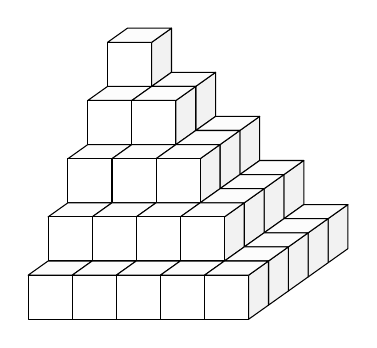
\begin{tikzpicture}[x=5.6mm,y=5.6mm,line cap=round,line join=round,line width=.38pt]
  \path[draw=black,fill=black!5] (2.8,5.28) -- (3.25,5.6) -- (3.25,6.6) -- (2.8,6.28) -- cycle;
  \path[draw=black,fill=black!1] (1.8,6.28) -- (2.8,6.28) -- (3.25,6.6) -- (2.25,6.6) -- cycle;
  \path[draw=black,fill=black!5] (3.8,4.28) -- (4.25,4.6) -- (4.25,5.6) -- (3.8,5.28) -- cycle;
  \path[draw=black,fill=black!1] (2.8,5.28) -- (3.8,5.28) -- (4.25,5.6) -- (3.25,5.6) -- cycle;
  \path[draw=black,fill=black!5] (4.8,3.28) -- (5.25,3.6) -- (5.25,4.6) -- (4.8,4.28) -- cycle;
  \path[draw=black,fill=black!1] (3.8,4.28) -- (4.8,4.28) -- (5.25,4.6) -- (4.25,4.6) -- cycle;
  \path[draw=black,fill=black!5] (5.8,2.28) -- (6.25,2.6) -- (6.25,3.6) -- (5.8,3.28) -- cycle;
  \path[draw=black,fill=black!1] (4.8,3.28) -- (5.8,3.28) -- (6.25,3.6) -- (5.25,3.6) -- cycle;
  \path[draw=black,fill=black!5] (6.8,1.28) -- (7.25,1.6) -- (7.25,2.6) -- (6.8,2.28) -- cycle;
  \path[draw=black,fill=black!1] (5.8,2.28) -- (6.8,2.28) -- (7.25,2.6) -- (6.25,2.6) -- cycle;
  \path[draw=black,fill=white] (1.8,5.28) -- (2.8,5.28) -- (2.8,6.28) -- (1.8,6.28) -- cycle;
  \path[draw=black,fill=black!1] (1.35,4.96) -- (2.35,4.96) -- (2.8,5.28) -- (1.8,5.28) -- cycle;
  \path[draw=black,fill=black!5] (3.35,3.96) -- (3.8,4.28) -- (3.8,5.28) -- (3.35,4.96) -- cycle;
  \path[draw=black,fill=black!1] (2.35,4.96) -- (3.35,4.96) -- (3.8,5.28) -- (2.8,5.28) -- cycle;
  \path[draw=black,fill=black!5] (4.35,2.96) -- (4.8,3.28) -- (4.8,4.28) -- (4.35,3.96) -- cycle;
  \path[draw=black,fill=black!1] (3.35,3.96) -- (4.35,3.96) -- (4.8,4.28) -- (3.8,4.28) -- cycle;
  \path[draw=black,fill=black!5] (5.35,1.96) -- (5.8,2.28) -- (5.8,3.28) -- (5.35,2.96) -- cycle;
  \path[draw=black,fill=black!1] (4.35,2.96) -- (5.35,2.96) -- (5.8,3.28) -- (4.8,3.28) -- cycle;
  \path[draw=black,fill=black!5] (6.35,0.96) -- (6.8,1.28) -- (6.8,2.28) -- (6.35,1.96) -- cycle;
  \path[draw=black,fill=black!1] (5.35,1.96) -- (6.35,1.96) -- (6.8,2.28) -- (5.8,2.28) -- cycle;
  \path[draw=black,fill=white] (1.35,3.96) -- (2.35,3.96) -- (2.35,4.96) -- (1.35,4.96) -- cycle;
  \path[draw=black,fill=white] (2.35,3.96) -- (3.35,3.96) -- (3.35,4.96) -- (2.35,4.96) -- cycle;
  \path[draw=black,fill=black!1] (0.9,3.64) -- (1.9,3.64) -- (2.35,3.96) -- (1.35,3.96) -- cycle;
  \path[draw=black,fill=black!1] (1.9,3.64) -- (2.9,3.64) -- (3.35,3.96) -- (2.35,3.96) -- cycle;
  \path[draw=black,fill=black!5] (3.9,2.64) -- (4.35,2.96) -- (4.35,3.96) -- (3.9,3.64) -- cycle;
  \path[draw=black,fill=black!1] (2.9,3.64) -- (3.9,3.64) -- (4.35,3.96) -- (3.35,3.96) -- cycle;
  \path[draw=black,fill=black!5] (4.9,1.64) -- (5.35,1.96) -- (5.35,2.96) -- (4.9,2.64) -- cycle;
  \path[draw=black,fill=black!1] (3.9,2.64) -- (4.9,2.64) -- (5.35,2.96) -- (4.35,2.96) -- cycle;
  \path[draw=black,fill=black!5] (5.9,0.64) -- (6.35,0.96) -- (6.35,1.96) -- (5.9,1.64) -- cycle;
  \path[draw=black,fill=black!1] (4.9,1.64) -- (5.9,1.64) -- (6.35,1.96) -- (5.35,1.96) -- cycle;
  \path[draw=black,fill=white] (0.9,2.64) -- (1.9,2.64) -- (1.9,3.64) -- (0.9,3.64) -- cycle;
  \path[draw=black,fill=white] (1.9,2.64) -- (2.9,2.64) -- (2.9,3.64) -- (1.9,3.64) -- cycle;
  \path[draw=black,fill=white] (2.9,2.64) -- (3.9,2.64) -- (3.9,3.64) -- (2.9,3.64) -- cycle;
  \path[draw=black,fill=black!1] (0.45,2.32) -- (1.45,2.32) -- (1.9,2.64) -- (0.9,2.64) -- cycle;
  \path[draw=black,fill=black!1] (1.45,2.32) -- (2.45,2.32) -- (2.9,2.64) -- (1.9,2.64) -- cycle;
  \path[draw=black,fill=black!1] (2.45,2.32) -- (3.45,2.32) -- (3.9,2.64) -- (2.9,2.64) -- cycle;
  \path[draw=black,fill=black!5] (4.45,1.32) -- (4.9,1.64) -- (4.9,2.64) -- (4.45,2.32) -- cycle;
  \path[draw=black,fill=black!1] (3.45,2.32) -- (4.45,2.32) -- (4.9,2.64) -- (3.9,2.64) -- cycle;
  \path[draw=black,fill=black!5] (5.45,0.32) -- (5.9,0.64) -- (5.9,1.64) -- (5.45,1.32) -- cycle;
  \path[draw=black,fill=black!1] (4.45,1.32) -- (5.45,1.32) -- (5.9,1.64) -- (4.9,1.64) -- cycle;
  \path[draw=black,fill=white] (0.45,1.32) -- (1.45,1.32) -- (1.45,2.32) -- (0.45,2.32) -- cycle;
  \path[draw=black,fill=white] (1.45,1.32) -- (2.45,1.32) -- (2.45,2.32) -- (1.45,2.32) -- cycle;
  \path[draw=black,fill=white] (2.45,1.32) -- (3.45,1.32) -- (3.45,2.32) -- (2.45,2.32) -- cycle;
  \path[draw=black,fill=white] (3.45,1.32) -- (4.45,1.32) -- (4.45,2.32) -- (3.45,2.32) -- cycle;
  \path[draw=black,fill=black!1] (0,1) -- (1,1) -- (1.45,1.32) -- (0.45,1.32) -- cycle;
  \path[draw=black,fill=black!1] (1,1) -- (2,1) -- (2.45,1.32) -- (1.45,1.32) -- cycle;
  \path[draw=black,fill=black!1] (2,1) -- (3,1) -- (3.45,1.32) -- (2.45,1.32) -- cycle;
  \path[draw=black,fill=black!1] (3,1) -- (4,1) -- (4.45,1.32) -- (3.45,1.32) -- cycle;
  \path[draw=black,fill=black!5] (5,0) -- (5.45,0.32) -- (5.45,1.32) -- (5,1) -- cycle;
  \path[draw=black,fill=black!1] (4,1) -- (5,1) -- (5.45,1.32) -- (4.45,1.32) -- cycle;
  \path[draw=black,fill=white] (0,0) -- (1,0) -- (1,1) -- (0,1) -- cycle;
  \path[draw=black,fill=white] (1,0) -- (2,0) -- (2,1) -- (1,1) -- cycle;
  \path[draw=black,fill=white] (2,0) -- (3,0) -- (3,1) -- (2,1) -- cycle;
  \path[draw=black,fill=white] (3,0) -- (4,0) -- (4,1) -- (3,1) -- cycle;
  \path[draw=black,fill=white] (4,0) -- (5,0) -- (5,1) -- (4,1) -- cycle;
\end{tikzpicture}%
}
